\documentclass[12pt,a4paper]{report}

\usepackage[utf8]{inputenc}
\usepackage[T1]{fontenc}
\usepackage{combelow}
\usepackage[romanian]{babel}
\usepackage{graphicx}
\usepackage{subfiles}
\usepackage{blindtext}
\usepackage[export]{adjustbox} 
\usepackage{geometry}
\usepackage[nottoc,notlot,notlof]{tocbibind}
\usepackage{indentfirst}
\usepackage{amsthm}
\usepackage{listings}
\usepackage{float}
\usepackage[toc,page]{appendix}
\usepackage{subcaption}
\usepackage{makeidx}
\usepackage{geometry}
\usepackage[verbose]{newunicodechar}
\usepackage{hyperref}
\usepackage{amsmath} 
\usepackage{xparse}
\usepackage[utf8]{inputenc}
\usepackage{chngcntr}
\usepackage{mathtools}
\usepackage[section]{placeins}
\graphicspath{{figures/}}
\usepackage{array}
\usepackage{afterpage}
\usepackage[font=small,labelfont=bf]{caption}

\usepackage{booktabs}
\usepackage{multirow}
\usepackage{color}

\usepackage{listings}
 
\definecolor{codegreen}{rgb}{0,0.6,0}
\definecolor{codegray}{rgb}{0.5,0.5,0.5}
\definecolor{codepurple}{rgb}{0.58,0,0.82}
\definecolor{backcolour}{rgb}{0.95,0.95,0.92}
 
\lstdefinestyle{mystyle}{
    backgroundcolor=\color{backcolour},   
    commentstyle=\color{codegreen},
    keywordstyle=\color{magenta},
    numberstyle=\tiny\color{codegray},
    stringstyle=\color{codepurple},
    basicstyle=\footnotesize,
    breakatwhitespace=false,         
    breaklines=true,                 
    captionpos=b,                    
    keepspaces=true,                 
    numbers=left,                    
    numbersep=5pt,                  
    showspaces=false,                
    showstringspaces=false,
    showtabs=false,                  
    tabsize=2
}
 
\lstset{style=mystyle}

\geometry{
	a4paper,
	total={170mm,257mm},
	left=25mm,
	top=25mm,
	bottom=25mm,
	right=25mm,
}

% Line spacing
\renewcommand{\baselinestretch}{1.5} 
\renewcommand\appendixtocname{Anexe}
\renewcommand\appendixname{Anexe}
\renewcommand\appendixpagename{Anexe}
\newcommand\blankpage{%
	\null
	\thispagestyle{empty}%
	\addtocounter{page}{-1}%
	\newpage}
\newcommand*\xor{\mathbin{\oplus}}


\DeclarePairedDelimiter\norm{\lVert}{\rVert}%
\DeclarePairedDelimiter\abs{\lvert}{\rvert}%

\graphicspath{{images/}{../images/}{figures/}{../figures/}}

\newunicodechar{ș}{\c{s}}
\newunicodechar{Ș}{\c{S}}
\newunicodechar{ț}{\c{t}}
\newunicodechar{Ț}{\c{T}}

\newtheorem{remark}{Observație}[chapter]
\newtheorem{definition}{Definiție}[chapter]
\newtheorem{lemma}{Lemă}[chapter]
\newtheorem{theorem}{Teoremă}[chapter]

\makeindex

\begin{document}

\afterpage{\blankpage}
\subfile{chapters/0_first_page}
\restoregeometry

\setcounter{page}{3}
\subfile{chapters/01_abstract_ro}

\newpage
\subfile{chapters/01_abstract_en}

\tableofcontents

\newpage
\addcontentsline{toc}{chapter}{\listfigurename}
\listoffigures

\newpage
\addcontentsline{toc}{chapter}{Listă de tabele}
\listoftables

\newpage
\addcontentsline{toc}{chapter}{Listă fragmente de cod}
\lstlistoflistings

\newpage\null\newpage
\chapter{Introducere}
\section{Motivație}

Volumul de date crește semnificativ de la an la an astfel până în 2020 se estimează că pentru fiecare persoană de pe planetă vor fi creați în fiecare secundă 1.7 MB de date, ceea ce înseamnă peste 13 milioane de GB creați în fiecare secundă în lume.

În 2018 în fiecare minut se vizionau peste 97 de mii de ore de conținut pe Netlfix. Peste 4.3 milioane de videoclipuri erau vizionate pe Youtube. Pe Spotify se ascultau 750 de mii de melodii, iar Amazon pregătea peste o mie de pachete \hyperlink{domo}{[1]}.

\vspace{5mm}

În România, Netflix pune la dispoziție 575 de filme și 208 seriale. În Regatul Unit sunt disponibile 2425 de filme și 542 de seriale, iar în Statele Unite Ale Americii sunt disponibile 2942 de filme și 629 de seriale \hyperlink{finder}{[2]}.

Amazon oferă cumpărătorilor o gamă cu un total de peste 119 milioane de produse, dintre care 44.2 milioane de cărți, 10.1 milioane de electronice sau 4.5 milioane de produse realizate manual \hyperlink{scrapehero}{[3]}.

\vspace{5mm}

În primă fază, cu cât volumul de date pus la dispoziție de o platforma este mai mare cu atât este mai mare și necesitatea unui sistem de recomandare care să vină în ajutorul utilizatorului final pentru a explora gama de produse oferită de respectiva platformă. Ulterior, acel sistem de recomandare se vrea a fi îmbunătățit astfel încât să ofere fiecărui utilizator o experiență cât mai personalizată prin care se recomande, în cazul platformelor de streaming video, conținut relevant pentru a fi consumat de utilizatorul final, sau în cazul platformelor de ecommerce, produse pe care utilizatorul ar fi dispus să le cumpere.

\vspace{5mm}

În majoritatea cazurilor sistemele de recomandare se bazeaza pe metadatele utilizatorilor, precum: regiunea, vârsta, genul, ce alte produse a accesat sau cumpărat și metadatele produselor: categoria din care face parte, ratingul acestuia. La acestea se pot adauga și alte informații precum: ce alte produse a apreciat un alt user cu un profil asemanător.

\section{Obiective propuse}
În majoritatea cazurilor primul contact pe care îl avem cu un clip de pe Youtube, cu un film sau serial de pe Netflix sau un produs de pe Amazon este contactul vizual cu imaginea de prezentare a acelui produs.

Astfel, prezenta lucrare de disertație are drept obiectiv principal introducerea în sistemul de recomandare de informații vizuale extrase din imaginile de prezentare ale produselor. Informațiile vizuale sunt reprezentate de clusterele create peste imaginile asociate produselor. Fiecare produs are o imagine de prezentare, iar fiecare imagine are un cluster caruia îi aparține din intervalul $[1, N]$ unde $N$ este corelat cu numărul de categori de produse din baza de date pe care se executa optimizarea. $N$ poate fi ales și pe baza altor raționamente.

Scopul final al acestei abordări fiind acela de a observa evoluția metricilor de evaluare, în cazul nostru acurateațea și precizia@k, atunci când informația vizuală este introdusă într-un sistem de recomandare, fiind singura informație prezentă exceptând matricea de interacțiuni, dar și cum se comportă un sistem de recomandare când primește această informație împreună cu alte informații, spre exemplu categoria unui articol.

\section{Structura lucrării}
Prezenta lucrare de disertație începe prin detalierea fundamentelor teoretice în capitolul II unde sunt prezentate teoriile ce stau la baza realizării acestei lucrări.

\newpage\null\newpage
\chapter{Fundamente teoretice}
\section{Sisteme de recomandare}

\subsection{Noțiuni generale}

Sistemele de recomandare au scopul de oferi sugestii de articole utilizatorilor unei platforme pe baza unor strategii. Un sistem de recomandare poate folosi una sau mai multe strategii de recomandare. 

În cazul în care se folosesc cel puțin două strategii, sistemul de recomandare devine un sistem de recomandare hibrid. Prin folosirea mai multor strategii se urmărește ca fiecare strategie să vină în completarea celorlalte cu avantajele sale.

De cele mai multe ori, în implementarea unui sistem de recomandare, se folosește tehnica de filtrare coloborativă împreună cu o altă strategie de recomandare \hyperlink{ErionCanoMaurizioMorisio}{[4]}.

\subsection{Strategii de recomandare}

\subsubsection*{Filtrarea coloborativă}

Filtrarea coloborativă se bazează pe faptul că utilizatorii care au în prezent preferințe similare vor avea și în viitor preferințe destul de similare. Această abordare folosește ratingurile pe care le dau utilizatorii sau oricare altă formă de a da un feedback, îmi place/nu îmi place, pentru a identifica preferințele comune dintre grupurile de utilizatori. Odată identificate preferințele se generează recomandări pe baza similarităților dintre utilizatori. 

Dezavantajul acestei strategii apare în momentul în care în sistem intră un nou utilizator. Datorită faptului că utilizatorul este nou, sistemul nu are un istoric al preferințelor lui, iar în consecință nu îl poate asigna unui grup de utilizatori pe baza preferințelor \hyperlink{ErionCanoMaurizioMorisio}{[4]}.

\begin{figure}[!h]
	\centering
	\includegraphics[max width=10cm,max height=10cm,keepaspectratio]{img_2_1}
	\caption[Filtrarea coloborativă]{Filtrarea coloborativă. Imagine preluată din \hyperlink{datameetsmedia}{[5]}.}
\end{figure} 

\subsubsection*{Filtrarea bazată pe conținut}

Filtrarea bazată pe conținut pleacă de la premisa că utiliztorii cărora le-au plăcut articole definite de anumite atribute în trecut, vor aprecia aceleași tip de articole și în viitor. Această abordare folosește atributele articolelor pentru a le compara cu profilul utilizatorilor și a oferi recomandări. Calitatea recomandărilor create folosind această strategie este influențată de setul de atribute ales pentru articole.

Similar cu filtrarea coloborativă și filtrarea bazată pe conținut prezintă dezavantaje în momentul în care în sistem intră un nou utilizator fără istoric \hyperlink{ErionCanoMaurizioMorisio}{[4]}.

\begin{figure}[!h]
	\centering
	\includegraphics[max width=10cm,max height=10cm,keepaspectratio]{img_2_2}
	\caption[Filtrarea bazată pe conținut]{Filtrarea bazată pe conținut. Imagine preluată din \hyperlink{datameetsmedia}{[5]}.}
\end{figure} 

\subsubsection*{Filtrarea demografică}

Filtrarea demografică folosește atribute precum vârsta, genul, educația, etc. pentru a identifica categoriile de utilizatori. Nu prezintă dezavantaje atunci când apar noi utilizatori în sistem și nu se folosește de ratinguri, sau alt sistem de feedback, pentru a face recomandări.

Dezavantajul este reprezentat de faptul că procesul de colectare al datelor demografice poate fi îngreunat de legislație fapt ce reprezintă o limitare a acestei metode \hyperlink{ErionCanoMaurizioMorisio}{[4]}.

\subsubsection*{Filtrarea bazată pe cunoștințe}

Filtrarea bazată pe cunoștințe folosește cunoștințele despre utilizatori și articole pentru a spune ce articole îndeplinesc cerințele utilizatorilor și genereaza recomandări în consecință. Filtrare bazată pe cunoștințe are la bază constrângeri și este capabilă să recomande chiar și articole complexe care nu sunt cumpărate atât de des, precum mașini sau case \hyperlink{ErionCanoMaurizioMorisio}{[4]}.

\subsection{Funcții de loss}

\subsubsection*{BPR: Bayesian Personalised Ranking}

Este o metodă ce se bazează pe feedback implicit (click-uri, ratinguri, achiziții). Exită multe metode ce se bazează pe acest feedback implicit, precum matrix factorization (MF), k-nearest-neighbor (kNN), însă acestea nu sunt optimizate pentru ranguri. Metoda de învățare este bazată pe gradientul descendent. Metoda este recomandată atunci când se dorește optimizarea acurateții.

Definim în continuare $U$ ca fiind mulțimea de utilizatori și $I$ ca fiind mulțimea de articole. Feedback-ul implicit este reprezentat de mulțimea $S \subseteq U \times I$. De asemenea, definim $I_u^+ := {i \in I:(u, i) \in S}$ și $U_i^+ := {u \in U:(u, i) \in S}$.

\begin{figure}[!h]
	\centering
	\includegraphics[max width=10cm,max height=10cm,keepaspectratio]{img_2_8}
	\caption[Matricea de interacțiuni]{Matricea de interacțiuni, mulțimea $S$. Imagine preluată din \hyperlink{SteffenRendleChristophFreudenthalerZenoGantnerLarsSchmidtThieme}{[9]}.}
\end{figure} 

O abordarea uzuală pentru recomandarea de articole este să fie prezis scorul $\hat{x}_{ui}$ care să reflecte preferința utilizatorului $u$ pentru articolul $i$. Apoi fiecare articol primește un rang după sortarea scorurilor.

Setul de antrenare este definit de mulțimea $D_S := \{(u,i,j)|i \in I_u^+ \wedge j \in I \setminus I_u^+\}$ unde $(u,i,j)$ înseamnă că utilizatorul $u$ preferă articolul $i$ în detrimentul articolului $j$.

\begin{figure}[!h]
	\centering
	\includegraphics[max width=10cm,max height=10cm,keepaspectratio]{img_2_9}
	\caption[Setul de antrenare]{Setul de antrenare. $+$ reprezintă articolele $i$ pe care utilizatorul le preferă în locul articolelor $j$, $-$ utilizatorul preferă articolele $j$ în loc de $i$, iar $?$ reprezintă lipsa informației despre acea interacțiune. Imagine preluată din \hyperlink{SteffenRendleChristophFreudenthalerZenoGantnerLarsSchmidtThieme}{[9]}.}
\end{figure} 

Criteriul de optimizare pentru pentru rangurile personalizate este definit după cum urmează:
\begin{align}
	BPR-OPT := \sum_{(u,i,j) \in D_S} \ln{\sigma(\hat{x}_{uij})} - \lambda_\Theta||\Theta||^2
\end{align}

unde $\sigma$ este funcția sigmoid, $\sigma(x) := \frac{1}{1+e^{-x}}$, $\Theta$ reprezintă vectorul parametru al modelului care definește interacțiunea dintre utilizatorul $u$, articolul $i$ și articolul $j$, iar $\lambda_\Theta$ reprezintă parametrii de regularizare.

\vspace{5mm}
Cu aceste definiți putem defini și procedura de învățare a $BPR$ după cum urmează.

\begin{figure}[!h]
	\centering
	\includegraphics[max width=10cm,max height=10cm,keepaspectratio]{img_2_10}
	\caption[Procedura de învățarea BPR]{Optimizarea modelului bazată metoda gradientului descendent cu parametrul de învățare $\alpha$ și regularizarea $\lambda_\Theta$. Imagine preluată din \hyperlink{SteffenRendleChristophFreudenthalerZenoGantnerLarsSchmidtThieme}{[9]}.}
\end{figure}

\vspace{5mm}
\subsubsection*{WARP: Weighted Approximate-Rank}

Această metodă își are originile în procesarea imaginilor și anume pentru un set de reprezentări ale unor imagini $x \in R^d$ și pentru un set de reprezentări ale unor adnotări $i \in \Upsilon = \{1, ..., Y\}$ - inidici intr-un dicționar cu posibile adnotări, metoda învață să mapeze imagini din spațiul reprezentărilor într-un spațiu comun $R^D$

\begin{align}
	\Phi_{I}(x):R^d \rightarrow R^D
\end{align}

în același timp învățând și mapări pentru adnotări în același spațiu

\begin{align}
	\Phi_{W}(i):{1,...,Y} \rightarrow R^D
\end{align}

Scopul principal fiind acela de a oferi ranguri posibilelor adnotări pentru o imagine dată astfel încât cel mai mare rang să descrie cel mai bine conținutul semnatic al imaginii. 

Modelul folosit este următorul:
\begin{align}
	f_{i}(x) = \Phi_{W}(i)^T \Phi_{I}(x)
\end{align}

Metoda învață să producă ranguri optimizate pentru primele adnotări din listă, ceea ce înseamnă că optimizează precizia@k.

În ceea ce privește funcția de eroare definim: $f(x) \in R^Y$ ce produce un scor pentru fiecare etichetă și unde $f_i(x)$ este valoarea etichetei $i$. Definim funcția de eroare pentru ranguri ca fiind:
\begin{align}
	err(f(x),y) = L(rank_y(f(x)))
\end{align}
unde $rank_y(f(x))$ este rangul etichetei corecte data de $f(x)$:
\begin{align}
	rank_y(f(x)) = \sum_{i \neq y}I(f_i(x) \geq f_y(x))
\end{align}
unde I este funcția indicator, iar $L(\cdot)$ transformă rangul în penalizare
\begin{align}
	L(k) = \sum_{j=1}^k\alpha_j, \quad cu \quad \alpha_1 \geq \alpha_2 \geq ... \geq 0.
\end{align}

$L(\cdot)$ poate lua diferite forme în funcție de ce se dorește a se optimiza: $\alpha_j=\frac{1}{Y-1}$ optimizează rangul mediu, $\alpha_j=1$ și $\alpha_{j>1}=0$ optimizează proporția de ranguri corecte aflate în top, iar valorile mari ale lui $\alpha$ optimizează primele $k$ în lista de ranguri\hyperlink{JasonWestonSamyBengioNicolasUsunier}{[8]}.

\vspace{5mm}

Cu definițiile prezentate mai sus putem descrie algoritmul acestei metode după cum urmează.

\begin{figure}[!h]
	\centering
	\includegraphics[max width=10cm,max height=10cm,keepaspectratio]{img_2_7}
	\caption[Online WARP Loss Optimization]{Online WARP Loss Optimization. Imagine preluată din \hyperlink{JasonWestonSamyBengioNicolasUsunier}{[8]}.}
\end{figure} 

\section{Rețele neurale convoluționale}

\subsection{Noțiuni generale}

Rețelele neurale convoluționale sunt foarte similare cu rețelele neurale fiind formate din neuroni ce învață ponderi ($w$) și baiasuri ($b$). Scopul rețelei convoluționale este de a primi o imagine la input și de a scoate la output un scor pentru fiecare clasă ce corespunde imaginii. 

Spre exemplu, la input se dă o imagine cu un autovehicul, iar rețeaua convoluțională poate spune că în imagine este o mașină în proporție de 80\%, un camion în proporție de 10\%, un avion în proporție de 6\%, o barcă în proporție de 3\% sau un cal în proporție de 1\%.

\begin{figure}[!h]
	\centering
	\includegraphics[max width=10cm,max height=10cm,keepaspectratio]{img_2_3}
	\caption[Exemplu rețea convoluțională]{Exemplu de rețea convoluțională care primește la input o imagine și produce la output o listă de clase ce pot descrie imaginea de input. Imagine preluată din \hyperlink{datameetsmedia}{[7]}.}
\end{figure} 

Rețelele convoluționale sunt compuse dintr-o secvență de layere ce poate fi împărțită în trei tipuri principale de layere \hyperlink{cs231n}{[7]}:

\begin{enumerate}
  \item Convolutional Layer este layerul de bază într-o rețea convoluțională. Parametrii acestui layer sunt reprezentați de filtre învățabile, unde fiecare filtru reprezintă o mică bucată din imaginea de input. De exemplu, un filtru pentru pentru acest layer poate avea dimensiunea de $5\times5\times3$, dimensiune ce reprezintă faptul că se iau 5 pixeli pe lațime și înălțime cu o adâncime de 3, unde adâncimea reprezintă canalele RGB. În continuare se glisează fiecare filtru peste input și se compune produsul dintre filtre și input la fiecare poziție. În urma acestei operații se produce un vector de activare 2-dimensional care reprezintă răspunsul filtrului la fiecare poziție. Altfel spun, rețeaua va învăța filtre care se activează atunci când sunt prezente anumite tipuri de caracteristici, precum culoarea sau orientarea.

\begin{figure}[!h]
	\centering
	\includegraphics[max width=10cm,max height=10cm,keepaspectratio]{img_2_4}
	\caption[Exemplu de filtru aplicat peste input]{Exemplu de filtru aplicat peste input într-un layer convoluțional. Imagine preluată din \hyperlink{datameetsmedia}{[7]}.}
\end{figure}   
  
  \item Pooling Layer reprezintă o practică des folosită între mai multe layere convoluționale succesive. Această operație reduce numărul de parametrii (dimensiunea), computațiile din rețea și controlează overfittingul. Se execută indepedent pe fiecare nivel al adâncimii unui input și pastrează valoarea maximă a acelei zone. Rezultatul este o zonă de caracteristicii mai mică dar care păstrează cea mai relevantă statistică.

\begin{figure}[!tbp]
  \begin{subfigure}[b]{0.4\textwidth}
    \includegraphics[width=\textwidth]{img_2_5}
    \caption{Reducerea dimensiunii.}
    \label{fig:f1}
  \end{subfigure}
  \hfill
  \begin{subfigure}[b]{0.4\textwidth}
    \includegraphics[width=\textwidth]{img_2_6}
    \caption{Filtrul de $2\times2$ aplicat ce păstrează valoarea maximă.}
    \label{fig:f2}
  \end{subfigure}
  \caption[Exemplu de pooling]{Exemplu de pooling. Imagine preluată din \hyperlink{datameetsmedia}{[7]}.}
\end{figure}
  
  \item Fully-Connected Layer este stratul în care caracteristicile sunt vectorizate pentru a putea fi folosite.
\end{enumerate}

\subsection{VGG}

\subsection{InceptionV3}

\subsection{ResNet}

\subsection{NASNet}



\section{Clustere}

\subsection{Noțiuni generale}

\subsection{K-nearest neighbors}


\newpage\null\newpage
\chapter{Descrierea soluției}
\section{Implementarea modelului de recomandare}
\subsection{Inițializarea}
În implementarea prezentei aplicații a fost folosit framework-ul de construcție a sistemelor de recomandare $LightFM$ \hyperlink{lightfm}{[21]} peste care am construit un wrapper. 
$LightFM$ conține o implemntare în Python a unor algoritmi de recomandare atât pentru feedback implicit cât și pentru feedback explicit. Metadatele articolelor și utilizatorilor pot fi încorporate intr-un algoritm tradițional de matrix factorization. Reprezentarea fiecărui articol și utilizator este o sumă a reprezentărilor latente ale caracteristicilor, ceea ce îi permite să generalizeze recomandările și către articole sau utilizatori noi.   

În continuare este prezentată inițializarea modelului de recomandare și explicația parametrilor folosiți atât cei definiți ca fiind maleabili cât și ceilalți parametrii puși la dispoziție de framework dar asupra cărora nu s-a intervenit în prezenta implementare:
\begin{lstlisting}[language=Python, caption=Definirea modelului de recomandare]
from lightfm import LightFM

__all__ = ['KingRec']


class KingRec(object):
    def __init__(self, no_components=50, loss='warp', learning_rate=0.05, alpha=0.02, scale=0.07):
        self.no_components = no_components
        self.loss = loss
        self.learning_rate = learning_rate
        self.item_alpha = alpha
        self.user_alpha = alpha * scale
        
        self.model = LightFM(no_components=no_components, 
        					 learning_rate=learning_rate, loss=loss,
                             item_alpha=self.item_alpha, 
                             user_alpha=self.user_alpha, 
                             random_state=2019)                       
\end{lstlisting}

Parametrii maleabili:
\begin{itemize}
  \item \textbf{no\_components}: numărul de componente reprezintă dimensiunea encodării latente a caracteristicilor utilizatorilor și articolelor. Spre exemplu, numărul de caracteristici pe fiecare user este de 1000 și avem 100 de utilizatori, ceea ce înseamnă o matrice de dimensiune $100 \times 1000$. Cu numărul de componente setat la 50, cum este prezentat în fragmentul de cod de mai sus, înseamnă ca numărul caracteristicilor pe fiecare user va fi redus la 50 de unde rezulta noua matrice a encodărilor latente a caracteristicilor de dimensiune $100 \times 50$.
  \item \textbf{learning\_rate}: reprezintă rata de învățare de start pe care o foloseștesistemul de recomandare. Această rată se poate schimba pe parcusul rulării ca urmare a faptului că s-a folosit algoritmul de optimizare Adagrad. Mai multe detalii despre acest algoritmi au fost prezentate în capitolul 2.2.3.
  \item \textbf{loss} funcția de eroare care poate fi una dintre următoarele funcții implementate: logistic, bpr, warp, warp-kos. Mai multe detalii despre funcțiile de eroare au fost prezentate în capitolul 2.1.3.
  \item \textbf{item\_alpha} penalizarea L2 norm a caracteristicilor articolelor. Este asignată direct din parametrul $alpha$.
  \item \textbf{user\_alpha} similar cu $item\_alpha$ și este rezultatul înmulțirii dintre parametrul $alpha$ și $scale$.
  \item \textbf{random\_state}: definește starea din care pleacă modelul de recomandare și este folosită de obicei pentru o reproducere mai ușoară a acelorași rezultate de la o rulare la alta.
\end{itemize}

Alți parametrii asupra carora nu s-a intervenit în prezenta implementare:
\begin{itemize}
	\item \textbf{k}: utilizat atunci când se folosește algoritmul k-OS și reprezintă al $k$-lea exemplu pozitiv ce va fi selectat din $n$ exemple pozitive pentru fiecare utilizator. Valoarea predefinită este setată la 5.
	\item \textbf{n}: utilizat atunci când se folosește algoritmul k-OS și reprezintă numărul maxim de exemple pozitive pentru fiecare actualizare. Valoarea predefinită este setată la 10.
	\item \textbf{learning\_schedule}: reprezintă algoritmul de optimizare și poate fi unul dintre adagrad sau adadelta. În experimentele realizate în această lucrare s-a folosit valoarea predefinită din model și anume adagrad.
	\item \textbf{max\_sampled}: reprezintă numărul maxim de exemple negative folosite în antrenarea cu WARP. Valoarea predefinită este setată la 10.
\end{itemize}

Odată definit modelul de recomandare putem crea o instanță a acestuia cu parametrii doriți dupa cum urmează:
\begin{lstlisting}[language=Python, caption=Instanțierea unui model]
from kingrec import KingRec

_, learning_rate, no_components, alpha, scaling = load_params(optimized_for='auc_clusters')

king_rec = KingRec(no_components=no_components, learning_rate=learning_rate, alpha=alpha, scale=scaling, loss='warp')
\end{lstlisting}
Această instanță va fi folosită în continuare în antrenarea și evaluarea modelului.
Funcția $load\_params$ încarcă parametrii optimi pentru pentru o anumită configurație. Mai multe detalii despre această optimizare a parametrilor este prezentată în capitolul 3.4.

\subsection{Antrenarea}
Cu o instanță a unui model creată putem antrena acel model pe un set de antrenare. Pentru a încărca un set de antrenare putem folosi funcția $init\_movielens$ care încarcă datasetul pus la dispoziție de grouplens \hyperlink{movielens}{[22]}. Mai multe detalii despre structura setului de date se pot găsi în capitolul 4.1.

\begin{lstlisting}[language=Python, caption=Funcția de inițializare a bazei de date]
def init_movielens(path, min_rating=0.0, k=3, item_features=None, cluster_n=18, model='vgg19')
\end{lstlisting}
unde:
\begin{itemize}
	\item \textbf{path}: este calea către folderul cu fișierele din setul de date;
	\item \textbf{min\_rating}: este ratingul minim pentru de la care vor fi construite interacțiunile dintre utilizatori și articole. Spre exemplu, dacă setăm un rating minim de $3.5$, mulțimea interacțiunilor pozitive va fi definită de acele interacțiuni pentru care utilizatorii au acordat cel puțin un rating de $3.5$, acestea fiind considerate interacțiuni pozitive. Restul interacțiunilor sunt considerate negative;
	\item \textbf{k}: este un parametru folosit doar pentru statisticii, în contextul de față prezintă câți utilizatori au minim $k$ interacțiuni în setul de date. Valoarea $k$ este folosită în metrica de evaluare $precizie@k$ după cum este prezentat în capitolul 3.1.1; 
	\item \textbf{item\_features}: poate lua una sau mai multe valori din mulțimea ${'genres', 'clusters'}$ și descrie tipurile de metadate ale articolelor care se doresc a fi prezente în setul de date. Desigur, acest parametru poate fi omis, astfel nefiind adăugate metadate suplimentare pe lângă interacțiunile dintre utilizatori și articole.
	\item \textbf{cluster\_n}: parametru folosit doar atunci când în $item\_features$ este prezentă valoarea $clusters$ și descrie în câte clastere trebuie să fie împărțite posterele filmelor. Clasterele sunt generate în prealabil și se găsesc în path-ul menționat;
	\item \textbf{model}: specifică modelul cu care au fost create posterele. Poate fi unul dintre următoarele: vgg19, inception\_v3, resnet50.
\end{itemize}
Funcția $init\_movielens$ returnează atât setul de date de antrenare cât și pe cel de testare. De asemenea, dacă este specificat prin parametrii returnează și metadatele filmelor.

Cu setul de date încarcat, putem face antrenarea cu funcția $fit$ sau $fit\_partial$. Diferența principală dintre cele două funcții este reprezentată de faptul că $fit\_partial$ reia antrenarea din starea curentă a modelului pe când $fit$ începe dintr-o stare nouă. 

\begin{lstlisting}[language=Python, caption=Antrenarea modelului]
model = king_rec.model
model.fit(interactions=train, item_features=item_features, epochs=epochs, verbose=True, num_threads=threads)
\end{lstlisting}
unde:
\begin{itemize}
	\item \textbf{interactions}: primește interacțiunile definite dintre utilizatori și filme;
	\item \textbf{item\_features}: reprezintă metadatele filmelor, dacă este cazul;
	\item \textbf{epochs}: reprezintă numărul de epoci pentru care vrem să facem antrenarea
	\item \textbf{verbose}: dacă este setat pe $True$ afișează progresul antrenării;
	\item \textbf{num\_threads}: numărul de threaduri pe care să fie executată antrenarea.
\end{itemize}

\subsection{Evaluarea}
Pe un model antrenat vom evalua două metrici pe setul de date de testare și anume \textit{acuratețea} și \textit{precizia@k}.
Prima dintre ele, \textit{acuratețea} este definită ca fiind probabilitatea ca un exemplu pozitiv ales în mod aleator să fie clasat mai sus în recomandări decât un exemplu negativ ales în mod aleator. Cea de-a doua, \textit{precizia@k} este definită de numărul de exemple pozitive aflate în primele $k$ recomandări.

Acuratețea poate fi calculată cu funcția $auc\_score$:
\begin{lstlisting}[language=Python, caption=Acuratețea unui model]
test_auc = auc_score(model, test_interactions, item_features=item_features, num_threads=threads).mean()
\end{lstlisting}
unde:
\begin{itemize}
	\item \textbf{model}: este modelul antrenat anterior;
	\item \textbf{test\_interactions}: reprezintă interacțiunile de test create cu funcția de inițializare a bazei de date;
	\item \textbf{item\_features}: reprezintă metadatele filmelor create cu funcția de intițializare a bazei de date;
	\item \textbf{num\_threads}: numărul de threaduri pe care se va executa evaluarea modelului.
\end{itemize}
Rezultatul produs este reprezentat de un scor de acuratețe pentru fiecare utilizator din setul de antrenare, iar rezultatul final al modelului este reprezentat de $mean$-ul tuturor rezultatelor de acuratețe per utilizator.

Precizia@k poate fi calculată cu funcția $precision\_at\_k$:

\begin{lstlisting}[language=Python, caption=Precizia@k a unui model]
test_precision = precision_at_k(model, test_interactions, item_features=item_features, k=k, num_threads=threads).mean()
\end{lstlisting}
unde:
\begin{itemize}
	\item \textbf{model, test\_interactions, item\_features și num\_threads}: descrise ca mai sus;
	\item \textbf{k}: numărul de recomandări peste care se calculează precizia pentru un utilizator.
\end{itemize}
Rezultatul produs este reprezentat de un scor de precizie@k pentru fiecare utilizator din setul de antrenare, iar rezultatul final al modelului este reprezentat de $mean$-ul tuturor rezultatelor de precizie per utilizator.

\section{Clasterizarea posterelor}
Procesul de clusterizare al posterelor presupune transformarea posterelor filmelor din imagini în clastere asociate fiecărui poster. Numărul total de clustere poate varia de la 2 până la 20 în cadrul acestei aplicații. De cele mai multe ori s-au folosit 18 clustere pentru a fi mapate 1 la 1 cu genurile filmelor.

Acest proces poate fi împărțit în două etape:
\begin{enumerate}
	\item Extragerea caracteristicilor din postere: în extragerea caracteristicilor din postere se folosesc mai multe rețele preantrenate printre care VGG16, VGG19, InceptionV3, ResNet50 sau NASNet. Mai multe detalii despre rețelele preantrenate pot fi găsite în capitolul 2.4. Folosim fiecare dintre rețelele menționate anterior până la stratul de glasificare, adică fără top-ul rețelelor, pentru a ne extrage doar caracteristicile din imagini. Imaginile în toate cele cinci rețele preantrenate întră cu dimensiunea fixă de $224 \times 224 \times 3$, inclusiv în rețeaua NASNet, chiar dacă aceasta poate accepta și dimensiuni mai mari. Fiecare film are câte un set de postere asociate, după cum este prezentat în capitolul 4.2. Din aceste seturi de postere alegem pentru fiecare film doar primul poster, poster pe care il trecem prin fiecare dintre rețelele menționate mai sus. Odată trecut prin fiecare rețea, salvăm caracteristicile aferente fiecărei rețele într-un fișier specific. Aceste fișiere sunt formate din id-ul filmului și caracteristicile extrase de rețeaua specifică din primul poster al fimului.
Funcția care se ocupă de acest proces este $extract\_images\_features()$ din modulul $extract\_features.py$.
	\item Creeare clusterelor pe baza caracteristicilor posterelor: odată create fișierele cu caracteristici pentru fiecare rețea putem rula funcția $explore\_clusters()$ din modulul $create\_clusters.py$. În acest moment fiecare fișier de caracteristici va fi parcurs, iar pentru fiecare dintre aceste fișiere vom crea între 2 și 20 de clastere. La final, toate aceste clastere vor fi salvate într-un fișier asociat rețelei preantrenate. Spre exemplu, rulam funcția de creeare clastere pentru rețeaua preantrenată vgg19. Funcția va citi din fișierul asociate rețelei caracteristicile posterelor pentru fiecare film. Cu aceste caracteristici va genera $2, 4, 6, ..., 20$ de clastere. La final toate clasterele sunt salvate într-un fișier specific rețelei sub forma: id film, id poster, cluster 2 (unde va fi trecut în care claster dintre cele două face parte posterul curent), cluster 4 (similar cu cluster 2), ..., cluster 20 (similar cu celelalte).
\end{enumerate}

\section{Construcția bazei de date}
Pentru construcția setului de date a fost folosită clasa \textit{Dataset} din framework-ul LightFM. Prima etapă în construirea de citirea ratingurilor date de utilizatori filmelor. Odată citite ratingurile aplicăm filtrarea de minim rating, dacă este cazul. Ratingurile astfel rămase compun matricea de interacțiune. Se face un split de $80\%$ date de antrenare și $20\%$ date de testare pe aceste interacțiuni.

Pe parte de caracteristici, se folosesc prestabilit atât pentru utilizatori cât și pentru filme matrici de identitate. Spre exemplu, daca avem 500 de utilizatori și 1000 de filme vom avea matricea de caracteristici a utilizatorilor de dimensiune $500 \times 500$ având valoarea 1 pe diagonală, iar matricea de caracteristici a filmelor de dimensiune $1000 \times 1000$, având de asemenea valorea 1 pe diagonală.

În continuare, în funcție de parametrii setați în funcția \textit{init\_movielens} se încarcă și celelalte caracterstici specifice filmelor. Dacă avem setate genurile pentru a fi încărcate în matricea de caracteristici atunci pentru fiecare film vom citi din fișierul specific genurilor din setul de date genurile acestora. Un film poate avea unul sau mai multe genuri. Pentru a introduce aceste caracteristici în matricea de caracteristici vom aplica \textit{one hot encoding} ceea ce presupune că pentru o mulțime de genuri de dimensiune $n$ vom codifica mulțimea genurilor asociate unui film într-un vector de prezență de dimensiune $n$. Ceea ce înseamnă că dacă avem o mulțime de șapte genuri, fie ele genul 1, genul 2, ..., genul 7. Dacă un film are genul 3 și genul 7 atunci vectorul lui de caracteristici asociate genurilor va fi următorul $[0, 0, 1, 0, 0, 0, 1]$.

De asemenea funcția \textit{init\_movielens} poate inițializa și clasterele aferente fiecărui film. Procesul este similar cu cel definit mai sus pentru transferul genurilor filmelor în matricea de caracteristici.

Cu cele de mai sus definite propune un exemplu ce înglobează descrierea de mai sus:
Fie un set de date cu 500 de utilizatori și 1000 de filme. Numărul total de genuri este de 18. Numărul total de clastere este corelat cu numărul total de genuri, ceea ce înseamnă că vom avea un total de 18 clastere.
\begin{figure}[!h]
	\centering
	\includegraphics[max width=10cm,max height=10cm,keepaspectratio]{img_3_1}
	\caption[Structura setului de date pentru utilizatori]{Structura setului de date pentru utilizatori.}
\end{figure} 

\begin{figure}[!h]
	\centering
	\includegraphics[max width=12cm,max height=12cm,keepaspectratio]{img_3_2}
	\caption[Structura setului de date pentru filme]{Structura setului de date pentru filme.}
\end{figure} 

\section{Optimizarea parametrilor modelului}

\begin{table}
\centering
\caption{Parametrii optimizați pentru modelul de recomandare pe tipuri de featureuri}
\label{table:1}
\resizebox{\textwidth}{!}{\begin{tabular}{|c|c|c|c|c|c|c|c|c|c|} 
\hline
\multirow{2}{*}{\textbf{Features}} & \multirow{2}{*}{\textbf{Loss}} & \multirow{2}{*}{\textbf{Optimize}} & \multicolumn{6}{c|}{\textbf{Optimal params}}                                                                    & \multirow{2}{*}{\textbf{Results}}  \\ 
\cline{4-9}
                          &                       &                           & \textbf{epochs} & \textbf{learning rate}         & \textbf{no components} & \textbf{item alpha}             & \textbf{scaling}               & \textbf{k os} &                           \\ 
\hline
None                      & warp                  & precision\_at\_k          & 141    & 0.043040683676705736  & 21            & 0.00541554967720231    & 0.014726505321746962  &      & \textbf{0.0920}                    \\ 
\hline
None                      & warp                  & auc\_score                & 93     & 0.013125743984880447  & 169           & 2.6154143367150727e-06 & 0.04382333041868763   &      & \textbf{0.9309}                    \\ 
\hline
None                      & warp-kos~             & precision\_at\_k          & 131    & 0.016193013939983108  & 131           & 0.014891088630376074   & 0.064172162850665     & 3    & 0.0915                    \\ 
\hline
None                      & warp-kos~             & auc\_score                & 136    & 0.025315151875417254  & 136           & 0.025315151875417254   & 0.0014438337247755933 & 5    & 0.9123                    \\ 
\hline
None                      & bpr                   & precision\_at\_k          & 145    & 0.011882573141627583  & 145           & 0.011882573141627583   & 0.008731133377250924  &      & 0.0818                    \\ 
\hline
None                      & bpr                   & auc\_score                & 100    & 0.38336028927731636   & 22            & 0.38336028927731636    & 0.6705805738529935    &      & 0.8738                    \\ 
\hline
genres                    & warp                  & precision\_at\_k          & 136    & 0.075490395178898     & 82            & 0.007065549151367718   & 0.00799962475267643   &      & \textbf{0.0990}                    \\ 
\hline
genres                    & warp                  & auc\_score                & 133    & 0.026238747910509397  & 193           & 0.0027085249085071626  & 0.07322973067589604   &      & \textbf{0.9384}                    \\ 
\hline
genres                    & warp-kos              & precision\_at\_k          & 106    & 0.04588316930944897   & 200           & 0.005855900490702136   & 0.09739540959401453   & 5    & 0.0968                    \\ 
\hline
genres                    & warp-kos              & auc\_score                & 128    & 0.031396765253117284  & 103           & 5.6689548595143295e-06 & 0.2992760477740958    & 5    & 0.9184                    \\ 
\hline
genres                    & bpr                   & precision\_at\_k          & 4      & 0.3988094699004826    & 174           & 0.00020130127273975477 & 0.9668511270812562    &      & 0.0793                    \\ 
\hline
genres                    & bpr                   & auc\_score                & 113    & 0.3787098755163822    & 20            & 1.412418076659026e-06  & 0.8846058572960187    &      & 0.8697                    \\ 
\hline
clusters                  & warp                  & precision\_at\_k          & 63     & 0.05647434188275842   & 98            & 0.0031993742820159436  & 0.0933642796909375    &      & \textbf{0.0938}                    \\ 
\hline
clusters                  & warp                  & auc\_score                & 42     & 0.0570326091236193    & 68            & 0.0029503539747277366  & 0.02563602355611453   &      & \textbf{0.9338}                    \\ 
\hline
clusters                  & warp-kos              & precision\_at\_k          & 111    & 0.12149792200676351   & 30            & 0.005138574720440468   & 0.22386245632097518   & 3    & 0.0900                    \\ 
\hline
clusters                  & warp-kos              & auc\_score                & 106    & 0.02060268158807219   & 153           & 0.0002768009203471932  & 0.01729102049278139   & 5    & 0.9139                    \\ 
\hline
clusters                  & bpr                   & precision\_at\_k          & 112    & 0.02783417000783745   & 53            & 0.043059513850700865   & 0.04509016538546181   &      & 0.0794                    \\ 
\hline
clusters                  & bpr                   & auc\_score                & 76     & 0.39695046755245167   & 20            & 3.559358324483847e-05  & 0.749186059016229     &      & 0.8656                    \\ 
\hline
genres, clusters          & warp                  & precision\_at\_k          & 96     & 0.1703221223672566    & 22            & 0.004206346506337412   & 0.041303781930858034  &      & \textbf{0.0980}                    \\ 
\hline
genres, clusters          & warp                  & auc\_score                & 120    & 0.027730397776550147  & 189           & 0.0011133373244076297  & 0.4922360335772573    &      & \textbf{0.9406}                    \\ 
\hline
genres, clusters          & warp-kos              & precision\_at\_k          & 83     & 0.07486946768773611   & 190           & 0.007918526926383375   & 0.012439949030585647  & 5    & 0.0916                    \\ 
\hline
genres, clusters          & warp-kos              & auc\_score                & 149    & 0.0374384222223599    & 98            & 6.392983080540728e-05  & 0.6204979332067604    & 5    & 0.9205                    \\ 
\hline
genres, clusters          & bpr                   & precision\_at\_k          & 19     & 0.0012968105572226996 & 140           & 9.939007330655304e-05  & 0.0011379548833006527 &      & 0.0597                    \\ 
\hline
genres, clusters          & bpr                   & auc\_score                & 98     & 0.3429430411358865    & 21            & 8.687526249607698e-06  & 0.7296865286380925    &      & 0.8681                    \\
\hline
\end{tabular}}
\end{table}

\begin{table}
\centering
\caption{Parametrii optimizați pentru modelul de recomandare pe tipuri de featureuri și modele de rețele preantrenate}
\label{table:2}
\resizebox{\textwidth}{!}{\begin{tabular}{|c|c|c|c|c|c|c|c|c|c|} 
\hline
\multirow{2}{*}{\textbf{Features} } & \multirow{2}{*}{\textbf{Loss }} & \multirow{2}{*}{\textbf{Optimize} } & \multicolumn{5}{c|}{\textbf{Optimal params}}                                                                      & \multirow{2}{*}{\textbf{Model} } & \multirow{2}{*}{\textbf{Results }}  \\ 
\cline{4-8}
                                    &                                 &                                     & \textbf{epochs} & \textbf{learning rate} & \textbf{no components} & \textbf{item alpha}   & \textbf{scaling}      &                                  &                                     \\ 
\hline
clusters                            & warp                            & precision\_at\_k                    & 232             & 0.07171978672352887    & 42                     & 0.006517845577815826  & 0.016142300018137722  & vgg19                            & 0.0935                              \\ 
\hline
clusters                            & warp                            & auc\_score                          & 89              & 0.018841927704689492   & 139                    & 0.0008662511914237855 & 0.2864763834214625    & vgg19                            & 0.9325                              \\ 
\hline
genres, clusters                    & warp                            & precision\_at\_k                    & 218             & 0.12470857345083873    & 73                     & 0.005478316990150038  & 0.04637764141484815   & vgg19                            & \textbf{0.0995}                              \\ 
\hline
genres, clusters                    & warp                            & auc\_score                          & 236             & 0.031860755009764305   & 139                    & 0.0010930770083784052 & 0.8362665749306415    & vgg19                            & 0.9413                              \\ 
\hline
clusters                            & warp                            & precision\_at\_k                    & 119             & 0.00852211930222011    & 192                    & 7.276515301192984e-05 & 0.027052254503857717  & inception\_v3                    & 0.0836                              \\ 
\hline
clusters                            & warp                            & auc\_score                          & 232             & 0.02981041359364386    & 84                     & 0.004287524090264805  & 0.040501994149651166  & inception\_v3                    & 0.9327                              \\ 
\hline
genres, clusters                    & warp                            & precision\_at\_k                    & 245             & 0.028963892665938032   & 43                     & 0.0006238083410955659 & 0.36579038826022736   & inception\_v3                    & 0.0905                              \\ 
\hline
genres, clusters                    & warp                            & auc\_score                          & 250             & 0.019411170816577752   & 136                    & 0.0008323333176050233 & 0.4767783602102349    & inception\_v3                    & \textbf{0.9425}                              \\ 
\hline
clusters                            & warp                            & precision\_at\_k                    & 88              & 0.07492160698420884    & 21                     & 0.004634987385145838  & 0.028198967823831238  & resnet50                         & \textbf{0.0953}                              \\ 
\hline
clusters                            & warp                            & auc\_score                          & 198             & 0.016780379637566917   & 169                    & 0.0012939223653296507 & 0.6692069103186539    & resnet50                         & \textbf{0.9342}                              \\ 
\hline
genres, clusters                    & warp                            & precision\_at\_k                    & 224             & 0.04214027912721876    & 186                    & 0.008676073688466915  & 0.0024915458462563605 & resnet50                         & 0.0970                              \\ 
\hline
genres, clusters                    & warp                            & auc\_score                          & 211             & 0.09767064566975311    & 48                     & 0.003428832598553235  & 0.11239835090728653   & resnet50                         & 0.9397                              \\
\hline
\end{tabular}}
\end{table}

\newpage\null\newpage
\chapter{Evaluarea experimentală}
\section{Bază de date filme}
În cadrul prezentei diserații a fost folosită ca bază de date pentru evaluarea experimentală baza oferita de grouplens \hyperlink{movielens}{[22]}. Aceștia pun la dispoziție mai multe seturi de date printre care:
\begin{enumerate}
	\item \textbf{MovieLens 20M Dataset}: conține 20 milioane de ratinguri oferite de 138 000 de utilizatori peste 27 000 de filme;
	\item \textbf{MovieLens 10M Dataset}: conține 10 milioane de ratinguri oferite de 72 000 de utilizatori peste 10 000 de filme;
	\item \textbf{MovieLens 1M Dataset}: conține 1 milion de ratinguri oferite de 6 000 de utilizatori peste 4 000 de filme.
\end{enumerate}

În evaluarea curentă a fost folosită cea mai recentă versiune de bază de date, actualizată la 9/2018, de dimensiune mică și anume \textit{ml-latest-small}. Această bază de date conține 100 000 de ratinguri și 3 600 de taguri aplicate peste 9 000 de filme de 600 de utilizatori. Această bază de date este un subset dintr-o bază de date cu 27 de milioane de ratinguri și 1 milion de taguri, aplicate peste 58 000 de filme de 280 000 de utilizatori.

Fiecare utilizator din \textit{ml-latest-small} a acordat ratinguri pentru cel puțin 20 de filme. Baza de date nu conține informații demografice, fiecare utilizator fiind reprezentat doar de un id.

Structura fișierelor din baza de date:
\begin{itemize}
	\item \textbf{ratings.csv}: fiecare linie din acest fișier reprezintă un rating dat de un utilizator unui film, fișierul având formatul $userId, movieId, rating, timestamp$, unde $timestamp$ reprezintă momentul de timp când a fost acordat ratingul. Fiecare rating este cuprins între 0 și 5, iar între ratinguri este unpas de 0.5;
	\item \textbf{movies.csv}: conține metadate despre filme precum titlul și genul. Formatul fișierului este următorul: $movieId, title, genres$. Titlul conține și anul de apariție a filmului sub forma \textit{Titlu (an)}. Genul poate fi unul sau mai multe dintre următoarele: \textit{Action, Adventure, Animation, Children's, Comedy, Crime, Documentary, Drama, Fantasy, Film-Noir, Horror, Musical, Mystery Romance, Sci-Fi, Thriller, War Western, (no genres listed)}.
	\item \textbf{links.csv}: conține referințele către site-urile movielens, imdb și themoviedb sub următorul format: $movieId,imdbId,tmdbId$.
	\item \textbf{tags.csv}: fiecare linie conține un tag aplicat de un utilizator unui film, fișierul având următorul format $userId,movieId,tag,timestamp$. Fiecare tag este reprezentat de un cuvânt sau de o scurtă frază.
\end{itemize}

\section{Bază de date postere}
În ceea ce privește baza de date pentru postere, aceasta a fost construită în cadrul dezvoltării prezentei lucrări cu ajutorul a două elemente: fișierul de \textit{links} din setul de date \textit{ml-latest-small} și cu API-ul pus la dispoziție de către platforma \textbf{themoviedb.org} \hyperlink{themoviedb}{[24]}.

Procesul de construcție a acestui set de postere pentru filme poate fi rezumat pe pași după cum urmează:
\begin{enumerate}
	\item \textbf{Pasul 1}: extragerea id-urilor filmelor aferente platformei themoviedb.org;
	\item \textbf{Pasul 2}: pentru fiecare film se face un request către API pentru a lua lista de postere pentru filmul curent;
	\item \textbf{Pasul 3}: având adresele posterelor pentru filmul curent, se descarcă și se salvează posterele la dimensiunea originală într-un folder specific filmului.
\end{enumerate}
Din punct de vedere al implementării putem menționa funcțiile:
\begin{lstlisting}[language=Python, caption=Construcția setul de date cu postere]
def get_tmdb_posters(tmdb_api_key, max_movie_posters=10):
    # pasul 1    
    tmdb_movies_id = get_tmdb_ids()
    # pasul 2 - 3
    download_images(tmdb_api_key, tmdb_movies_id, max_movie_posters)

# unde download_images are urmatoarea definitie:
def download_images(tmdb_api_key, tmdb_movies_id, max_movie_posters=10):
\end{lstlisting}
unde:
\begin{itemize}
	\item \textbf{tmdb\_api\_key} este api key-ul unic asociat unui cont pe platforma themoviedb.org care a solicitat acces la API-ul platformei;
	\item \textbf{max\_movie\_posters} definește care este numărul maxim de postere care va fi descărcat pentru un film. Numărul de postere descărcate poate fi mai mic în cazul în care nu sunt cel puțin max\_movie\_posters.
\end{itemize}

\begin{figure}[!tbp]
  \begin{subfigure}[b]{0.3\textwidth}
    \includegraphics[width=9cm,height=5cm,keepaspectratio]{img_4_1}
  \end{subfigure}
  \hfill
  \begin{subfigure}[b]{0.3\textwidth}
    \includegraphics[width=9cm,height=5cm,keepaspectratio]{img_4_2}
  \end{subfigure}
  \hfill
  \begin{subfigure}[b]{0.3\textwidth}
    \includegraphics[width=9cm,height=5cm,keepaspectratio]{img_4_3}
  \end{subfigure}
  \hfill
  \begin{subfigure}[b]{0.3\textwidth}
    \includegraphics[width=9cm,height=5cm,keepaspectratio]{img_4_4}
  \end{subfigure}
  \hfill
  \begin{subfigure}[b]{0.3\textwidth}
    \includegraphics[width=9cm,height=5cm,keepaspectratio]{img_4_5}
  \end{subfigure}
  \hfill
  \begin{subfigure}[b]{0.3\textwidth}
    \includegraphics[width=9cm,height=5cm,keepaspectratio]{img_4_6}
  \end{subfigure}
  \caption[Exemple de postere]{Exemplu de postere pentru filmul Paddington 2.}
\end{figure}

\section{Rezultate clusterizare postere}

\subsection{Sanity check}
Pentru testarea validității clasterelor un test de sanity check în care s-au luat opt filme și s-a încercat clasificarea lor în șapte clastere folosind caracteristicile extrase din rețelele preantrenate VGG16, VGG19, InceptionV3, ResNet50 și NASNet, clasterele create cu kNN iar evaluarea este făcută atât vizual cât și prin urmărirea evoluției metricii silhouette de la 2 la 7 clastere. Posterele de input pentru sanity check sunt prezentate în figura 4.2.
\begin{figure}[!tbp]
  \centering
  \begin{subfigure}[b]{0.48\textwidth}
    
\includegraphics[width=\textwidth]{img_4_7}
  \end{subfigure}
  \hfill
  \begin{subfigure}[b]{0.48\textwidth}
    
\includegraphics[width=\textwidth]{img_4_8}
  \end{subfigure}
    \hfill
  \begin{subfigure}[b]{0.48\textwidth}
    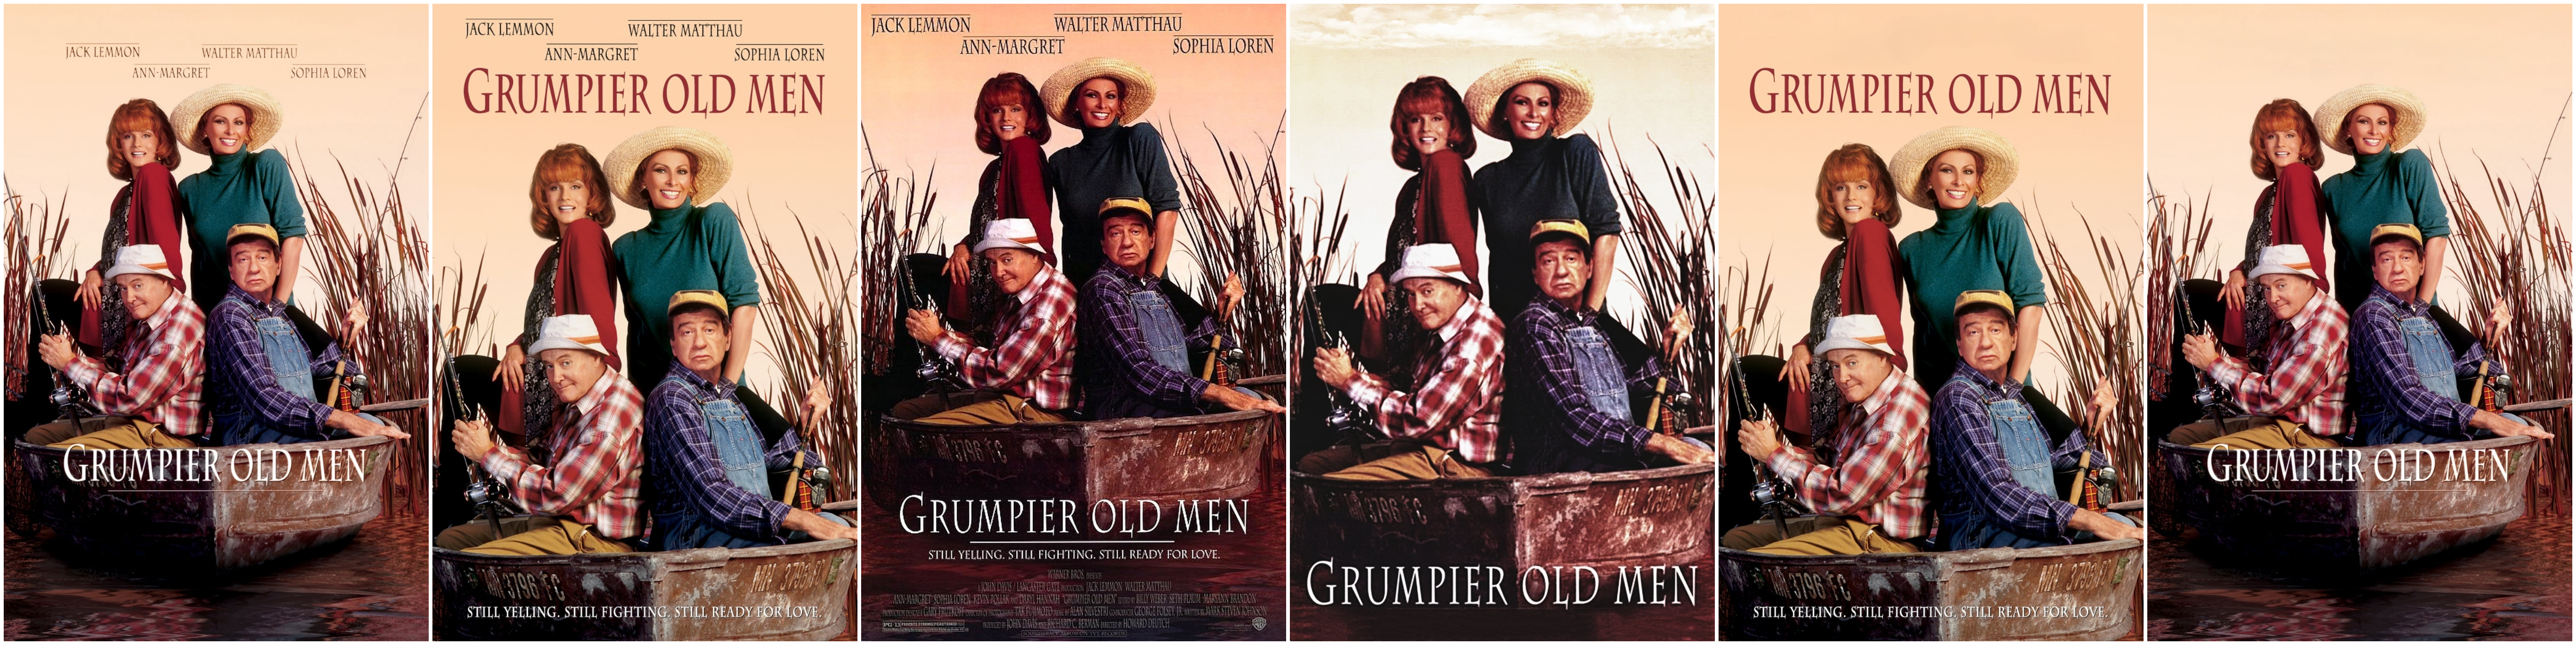
\includegraphics[width=\textwidth]{img_4_9}
  \end{subfigure}
  \hfill
  \begin{subfigure}[b]{0.48\textwidth}
    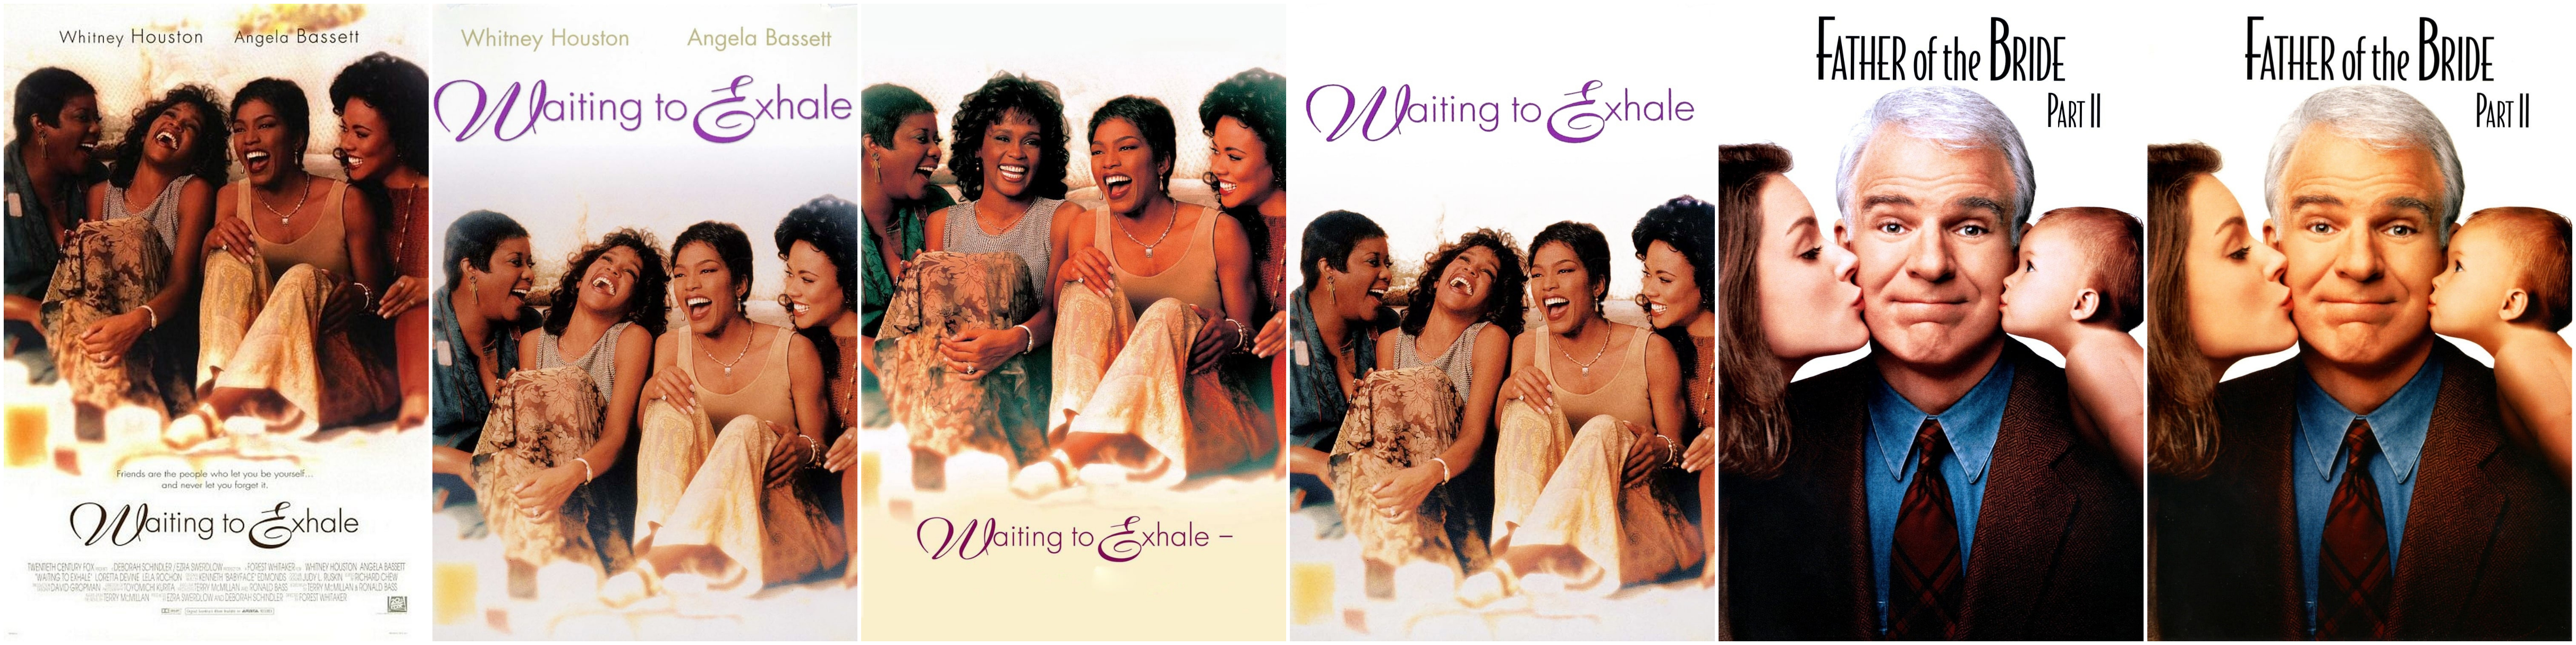
\includegraphics[width=\textwidth]{img_4_10}
  \end{subfigure}
  \hfill
  \begin{subfigure}[b]{0.48\textwidth}
    \includegraphics[width=\textwidth]{img_4_11}
  \end{subfigure}
  \hfill
  \begin{subfigure}[b]{0.48\textwidth}
    \includegraphics[width=\textwidth]{img_4_12}
  \end{subfigure}
    \hfill
  \begin{subfigure}[b]{0.48\textwidth}
    \includegraphics[width=\textwidth]{img_4_13}
  \end{subfigure}
    \hfill
  \begin{subfigure}[b]{0.48\textwidth}
    \includegraphics[width=\textwidth]{img_4_14}
  \end{subfigure}
      \hfill
  \begin{subfigure}[b]{0.3\textwidth}
    \includegraphics[width=\textwidth]{img_4_15}
  \end{subfigure}
  \caption[Postere input sanity check]{Posterele de input pentru sanity check.}
\end{figure}

Din punct de vedere al metricii de evaluare silhouette rezultatele se prezintă după cum urmează în figura 4.3.
\begin{figure}[!h]
	\centering
	\includegraphics[max width=12cm,max height=12cm,keepaspectratio]{img_4_16}
	\caption[Silhouette score pentru clasterele din sanity check]{Silhouette score pentru clasterele din sanity check.}
\end{figure} 
După cum se oberservă reţelele InceptionV3 şi NASNet pare a ieşi
mereu mai bine decât celelalte, cu un avantaj al reţelei InceptionV3. Această observaţie
fiind valabile pentru toate clasterele de la 2 la 7. Toate celelalte reţele sunt destul de
apropiate în rezultate în special începând cu clasterul 3 şi mai puţin la clasterul 2. Toate
celelalte reţele, cu excepţia ResNet50 au fluctuaţii. ResNet50 este singura care păstrează
în mod continuu trendul ascendent de la clasterul 2 până la clasterul 7.

Din punct de vedere vizual, rezultatatele clasterelor sunt prezentate în figurile 4.4 - 4.8.
\begin{figure}[!tbp]
  \centering
  \begin{subfigure}[b]{0.45\textwidth}
    \includegraphics[width=\textwidth]{img_vgg16_c1}
    \caption{claster 1}
  \end{subfigure}
  \hfill
  \begin{subfigure}[b]{0.45\textwidth}
    \includegraphics[width=\textwidth]{img_vgg16_c2}
    \caption{claster 2}
  \end{subfigure}
   \hfill
  \begin{subfigure}[b]{0.45\textwidth}
    \includegraphics[width=\textwidth]{img_vgg16_c3}
    \caption{claster 3}
  \end{subfigure}
  \hfill
  \begin{subfigure}[b]{0.45\textwidth}
    \includegraphics[width=\textwidth]{img_vgg16_c4}
    \caption{claster 4}
  \end{subfigure}
  \hfill
  \begin{subfigure}[b]{0.45\textwidth}
    \includegraphics[width=\textwidth]{img_vgg16_c5}
    \caption{claster 5}
  \end{subfigure}
  \hfill
  \begin{subfigure}[b]{0.45\textwidth}
    \includegraphics[width=\textwidth]{img_vgg16_c6}
    \caption{claster 6}
  \end{subfigure}
    \hfill
  \begin{subfigure}[b]{0.45\textwidth}
    \includegraphics[width=\textwidth]{img_vgg16_c7}
    \caption{claster 7}
  \end{subfigure}
  \caption[Rezultate sanity check pentru rețeaua VGG16]{Rezultate sanity check pentru rețeaua VGG16}
\end{figure}

\begin{figure}[!tbp]
  \centering
  \begin{subfigure}[b]{0.50\textwidth}
    \includegraphics[width=\textwidth]{img_vgg19_c1}
    \caption{claster 1}
  \end{subfigure}
  \hfill
  \begin{subfigure}[b]{0.50\textwidth}
    \includegraphics[width=\textwidth]{img_vgg19_c2}
    \caption{claster 2}
  \end{subfigure}
   \hfill
  \begin{subfigure}[b]{0.50\textwidth}
    \includegraphics[width=\textwidth]{img_vgg19_c3}
    \caption{claster 3}
  \end{subfigure}
  \hfill
  \begin{subfigure}[b]{0.50\textwidth}
    \includegraphics[width=\textwidth]{img_vgg19_c4}
    \caption{claster 4}
  \end{subfigure}
  \hfill
  \begin{subfigure}[b]{0.50\textwidth}
    \includegraphics[width=\textwidth]{img_vgg19_c5}
    \caption{claster 5}
  \end{subfigure}
  \hfill
  \begin{subfigure}[b]{0.50\textwidth}
    \includegraphics[width=\textwidth]{img_vgg19_c6}
    \caption{claster 6}
  \end{subfigure}
    \hfill
  \begin{subfigure}[b]{0.50\textwidth}
    \includegraphics[width=\textwidth]{img_vgg19_c7}
    \caption{claster 7}
  \end{subfigure}
  \caption[Rezultate sanity check pentru rețeaua VGG19]{Rezultate sanity check pentru rețeaua VGG19}
\end{figure}

\begin{figure}[!tbp]
  \centering
  \begin{subfigure}[b]{0.45\textwidth}
    \includegraphics[width=\textwidth]{img_inceptionv3_c1}
    \caption{claster 1}
  \end{subfigure}
  \hfill
  \begin{subfigure}[b]{0.45\textwidth}
    \includegraphics[width=\textwidth]{img_inceptionv3_c2}
    \caption{claster 2}
  \end{subfigure}
   \hfill
  \begin{subfigure}[b]{0.45\textwidth}
    \includegraphics[width=\textwidth]{img_inceptionv3_c3}
    \caption{claster 3}
  \end{subfigure}
  \hfill
  \begin{subfigure}[b]{0.45\textwidth}
    \includegraphics[width=\textwidth]{img_inceptionv3_c4}
    \caption{claster 4}
  \end{subfigure}
  \hfill
  \begin{subfigure}[b]{0.45\textwidth}
    \includegraphics[width=\textwidth]{img_inceptionv3_c5}
    \caption{claster 5}
  \end{subfigure}
  \hfill
  \begin{subfigure}[b]{0.45\textwidth}
    \includegraphics[width=\textwidth]{img_inceptionv3_c6}
    \caption{claster 6}
  \end{subfigure}
    \hfill
  \begin{subfigure}[b]{0.45\textwidth}
    \includegraphics[width=\textwidth]{img_inceptionv3_c7}
    \caption{claster 7}
  \end{subfigure}
  \caption[Rezultate sanity check pentru rețeaua InceptionV3]{Rezultate sanity check pentru rețeaua InceptionV3}
\end{figure}

\begin{figure}[!tbp]
  \centering
  \begin{subfigure}[b]{0.45\textwidth}
    \includegraphics[width=\textwidth]{img_resnet50_c1}
    \caption{claster 1}
  \end{subfigure}
  \hfill
  \begin{subfigure}[b]{0.45\textwidth}
    \includegraphics[width=\textwidth]{img_resnet50_c2}
    \caption{claster 2}
  \end{subfigure}
   \hfill
  \begin{subfigure}[b]{0.45\textwidth}
    \includegraphics[width=\textwidth]{img_resnet50_c3}
    \caption{claster 3}
  \end{subfigure}
  \hfill
  \begin{subfigure}[b]{0.45\textwidth}
    \includegraphics[width=\textwidth]{img_resnet50_c4}
    \caption{claster 4}
  \end{subfigure}
  \hfill
  \begin{subfigure}[b]{0.45\textwidth}
    \includegraphics[width=\textwidth]{img_resnet50_c5}
    \caption{claster 5}
  \end{subfigure}
  \hfill
  \begin{subfigure}[b]{0.45\textwidth}
    \includegraphics[width=\textwidth]{img_resnet50_c6}
    \caption{claster 6}
  \end{subfigure}
    \hfill
  \begin{subfigure}[b]{0.45\textwidth}
    \includegraphics[width=\textwidth]{img_resnet50_c7}
    \caption{claster 7}
  \end{subfigure}
  \caption[Rezultate sanity check pentru rețeaua ResNet50]{Rezultate sanity check pentru rețeaua ResNet50}
\end{figure}

\begin{figure}[!tbp]
  \centering
  \begin{subfigure}[b]{0.48\textwidth}
    \includegraphics[width=\textwidth]{img_nasnet_c1}
    \caption{claster 1}
  \end{subfigure}
  \hfill
  \begin{subfigure}[b]{0.48\textwidth}
    \includegraphics[width=\textwidth]{img_nasnet_c2}
    \caption{claster 2}
  \end{subfigure}
   \hfill
  \begin{subfigure}[b]{0.48\textwidth}
    \includegraphics[width=\textwidth]{img_nasnet_c3}
    \caption{claster 3}
  \end{subfigure}
  \hfill
  \begin{subfigure}[b]{0.48\textwidth}
    \includegraphics[width=\textwidth]{img_nasnet_c4}
    \caption{claster 4}
  \end{subfigure}
  \hfill
  \begin{subfigure}[b]{0.48\textwidth}
    \includegraphics[width=\textwidth]{img_nasnet_c5}
    \caption{claster 5}
  \end{subfigure}
  \hfill
  \begin{subfigure}[b]{0.48\textwidth}
    \includegraphics[width=\textwidth]{img_nasnet_c6}
    \caption{claster 6}
  \end{subfigure}
    \hfill
  \begin{subfigure}[b]{0.48\textwidth}
    \includegraphics[width=\textwidth]{img_nasnet_c7}
    \caption{claster 7}
  \end{subfigure}
  \caption[Rezultate sanity check pentru rețeaua NASNet]{Rezultate sanity check pentru rețeaua NASNet}
\end{figure}

După cum se observă, din punct de vedere vizual doar rețeaua ResNet50 reușește să treacă acest sanity check clasificând sașe filme în șase clastere diferite, iar două filme în același claster. Din punct de vedere vizual posterele celor două filme clasificate în același cluster sunt destul de similare având în prim plan mai multe persoane, predominant începând cu partea de jos a posterelor, iar in partea de sus fiind conținut alb, în general, cu text.

Observăm că deși InceptionV3 și NASNet aveau scoruri mai mari pe coeficientul silhouette, rețeaua ResNet50 are rezultate vizuale mai bune pe sanity check. De remarcat corelația dintre faptul că rețeaua ResNet50 este singura a cărui coeficient silhouette creștea de la un claster la altul, ceea ce înseamnă că acele clastere deveneau din ce în ce mai bune pe măsură ce ne apropiam de numărul de clastere din realitate.

\subsection{Rezultate generale}
Pentru evaluarea clasterelor pe toate pe toate posterele filmelor, aproximativ 9 000, au fost eliminate din evaluare rețelele VGG16 și NASNet în baza rezultatelor prezentate în tabelul 3.1, în cazul rețelei VGG16 și a costului de memorie și timp de execuție din timpul experimentelor, în cazul rețelei NASNet.
\begin{figure}[!h]
	\centering
	\includegraphics[max width=12cm,max height=12cm,keepaspectratio]{img_4_17}
	\caption[Scorul silhouette pe setul de date de postere]{Scorul silhouette pe setul de date de postere.}
\end{figure} 
Se observă că rețeaua InceptionV3 are scorurile pentru toate clasterele de la 2 la 20 pozitive. Rețelele ResNet50 și VGG19 sunt negative, însă apropiate de 0 cu un avantaj de scoruri mai bune pentru rețeaua ResNet50.

\section{Rezultate sistem de recomandare}
În continuare vom studia rezultatele obținute de metricile de evaluare \textbf{precizie@k} și \textbf{acuratețe} pe timp de antrenare în epoci, pe metadate folosite în antrenarea modelului și pe tipuri de rețele preantrenate cu care au fost generate clasterele posterelor. Toate mențiunile către parametrii optimi pentru o anumite configurație se referă la parametrii prezentați în tabelele 3.1 și 3.2.

Rezultatele metricii de acuratețe sunt prezentate în figura 4.10. Aceste rezultate sun obținute utilizând parametrii optimi din tabelul 3.1. Reamintim că toate clasterele folosite pentru obținerea parametrilor optimi din din acest tabel au fost create folosind rețeaua VGG19.
\begin{figure}[!h]
	\centering
	\includegraphics[max width=12cm,max height=12cm,keepaspectratio]{img_4_18}
	\caption[Comparație acuratețea modelului cu parametrii optimi pe tipuri de metadate]{Comparație acuratețea modelului cu parametrii optimi pe tipuri de metadate.}
\end{figure}
Principalele concluzii pe care e putem trage pe baza acestui grafic sunt următoarele:
\begin{itemize}
	\item modelul fără metadate are un start mai bun decât decât modelul cu genuri sau modelul cu genuri și cu clastere, însă acesta nu urcă prea mult pe durata perioadei de antrenare, astfel ajungând să aibă cel mai slab rezultat dintre toate cele patru variante de model testate;
	\item modelul cu metadatele de genuri are un start destul de slab, fiind mai bun doar de modelul în care se folosesc atât genurile cât și clasterele, însă, până la final, acest model obține un rezultat bun și apropiat de rezultatul modelului cu genuri și clastere. O altă mențiune importantă ar fi că acest model are cea mai mare durată de antrenare față de toate celelalte modele;
	\item modelul cu metadatele de clastere are cel mai bun start și în același timp cea mai scurtă perioadă de antrenare pentru a obține cel mai optim rezultat dintre toate modelele testate. Acuratețea obținută de acest model este peste acurateșea obținută de modelul fără metadate dar sub cea obținută de modelul cu genuri însă destul de apropiată de aceasta;
	\item cel mai bun rezultat din acest experiment este obținut de modelul în care se folosesc atât metadatele de genuri cât și cele de clastere. Modelul are cel mai slab start însă cel mai bun rezultat final. Observăm că modul în care este obținut rezultatul este o combinație a avantajelor modelelor cu metadate de genuri și clastere. Pe de-o parte, acuratețea crește semnificativ față de modelul fără metadate și este apropiată de acuratețea modelului cu genuri. Pe de alta parte timpul de necesar obținerii acelui rezultat optim este mai scăzut decât la modelul cu genuri, timp influențat de metadatele de clastere.
\end{itemize}
Concluzia principală a acestui experiment este că un model ce conține genuri și clastere are o performanță de până la $1\%$ în plus față de modelul fără metadate și mai mare față de oricare alt model, iar timpul necesar pentru obținerea acestei performanțe este mai mic în comparație cu cel mai apropiat model din punct de vedere al metricii evaluate.

Pentru a avea o imagine mai completă de cum se pot comporta aceste modele în timp am eliminat parametrul optimi găsit pe numărul de epoci și l-am setat pentru fiecare model la un număr de 300 de epoci. Iar după cum se observă în figura 4.11 toate modele după punctul optim în care ating performanța maximă încep să scadă. Modelele fără metadate, cu metadatele de genuri și cu metadatele de clastere au o scădere destul de lină în timp, pe când scăderea este mai acelărată în cazul modelului ce folosește metadatele de clastere față de celelalte modele. 
Acest al doilea grafic conturează și mai bine o concluzie pe care o putem trage despre modelul cu clastere și anume: acesta atinge performanța maximă foarte repede din punct de vedere al timpului de execuție în comparație cu oricare al model testat în cadrul acestei lucrări, iar din acel moment în care a fost obținută performanța maximă nu mai este recomandată prelungirea procesului de antrenare scăderea care va urma după punctul maxim va fi foarte acelărată.
\begin{figure}[!h]
	\centering
	\includegraphics[max width=12cm,max height=12cm,keepaspectratio]{img_4_19}
	\caption[Comparație acuratețea modelului cu parametrii optimi pe tipuri de metadate cu număr setat de epoci]{Comparație acuratețea modelului cu parametrii optimi pe tipuri de metadate cu număr setat de epoci.}
\end{figure}

\newpage\null\newpage
\chapter*{Concluzii}
\subsection*{Concluziile generale}

Ca urmare a rezultatelor prezentate în capitolul precedent putem afirma că prezenta lucrare de disertație și-a atins scopul și anume acela de a aduce o îmbunătățirea sistemelor de recomandare pentru filme folosind informația vizuală din postere. 
Scorul de la care a plecat sistemul de recomandare fără metadate incluse este de $93.13\%$ în cazul acurateții și de $9.26\%$ în cazul preciziei. Acest scor urcă până la $93.45\%$ acuratețe în cazul în care se adaugă informația vizuală de clustere creată cu rețeaua preantrenată ResNet50, iar cel de precizie urcă până la $9.63\%$ folosind rețeaua VGG19. Dacă informația vizuală este adăugată alături de genurile filmelor în metadate atunci scorurile ajung până la $94.22\%$ pentru acuratețe folosind rețeaua InceptionV3 și $10.05\%$ pentru precizie folosind rețeaua VGG19.

Se observă că în cazul acurateții rețeaua preantrenată optimă poate să difere în funcție de ce alte metadate sunt incluse în sistem, ResNet50 dacă sunt prezente doar posterele și InceptionV3 dacă sunt prezente atât posterele cât și genurile filmelor. Pe când în cazul preciziei rețeaua preantrenată optimă râmăne acceași indiferent de metadatele folosite și anume VGG19.

O altă observație importantă de făcut este faptul că în general clusterele pe postere tind să scadă timpul necesar de antrenare după cum se poate observa în figurile din capitolul precedent. 

Astfel, față de modelul de bază dacă introducem posterele ca informație vizuală metricile de acuratețe și precizie, cu parametrii optimi identificați, urcă până la $93.45\%$ pentru acuratețe și $9.63\%$ pentru precizie ceea ce înseamnă o îmbunătățire a modelului de recomandare de $0.32\%$ pe acuratețe și $0.42\%$ pe precizie.

Dacă posterele sunt combinate cu genurile filmelor, atunci scorurile metricilor, cu parametrii optimi identificați, urcă până la $94.22\%$ în cazul acurateții și $10.05\%$ în cazul preciziei ceea ce înseamnă o îmbunătățire a modelului de recomandare de $1.09\%$ pe acuratețe și $0.82\%$ pe precizie. 

\subsection*{Direcții viitoare de dezvoltare}
Abordarea prezentată în cadrul acestei lucrări poate fi ușor generalizată și către alte zone. Spre exemplu, aceași idee poate funcționa și în cazul unui sistem de recomandare pe o platformă de ecommerce deoarece fiecare articol de pe site are un set de imagini reprezentative, iar din acel set de imagini se pot creea clustere care pot sa fie relative la numărul de categorii de pe site. Un cazul unui site de haine, din nou, imaginile articolelor sunt reprezentative. La fel de bine ar putea funcționa și pe un site de mâncare. 

Situațiile în care este posibil ca rezultatele să nu fie neapărat satisfăcătoare ar putea fi reprezentate de siteurile cu cărți, deoarece coperțile cărților nu sunt la fel de reprezentative pentru acel produs precum sunt posterele filmelor sau imaginile cu haine.

\begin{thebibliography}{9}

	\bibitem{domo}
	\hypertarget{domo}{} 
	Data never sleeps 6.0
	\\\texttt{\url{https://www.domo.com/learn/data-never-sleeps-6}}
	
	\bibitem{finder}
	\hypertarget{finder}{} 
	Netflix International: What movies and TV shows can I watch, and where can I watch them?
	\\\texttt{\url{https://www.finder.com/global-netflix-library-totals}}

	\bibitem{scrapehero}
	\hypertarget{scrapehero}{} 
	How Many Products Does Amazon Sell? – April 2019
	\\\texttt{\url{https://www.scrapehero.com/number-of-products-on-amazon-april-2019/}}
	
	\bibitem{ErionCanoMaurizioMorisio}
	\hypertarget{ErionCanoMaurizioMorisio}{} 
	Erion Çano, Maurizio Morisio.
	\textit{\href{https://arxiv.org/abs/1901.03888}{Hybrid Recommender Systems: A Systematic Literature Review}}.
	Intelligent Data Analysis, vol. 21, no. 6, pp. 1487-1524, 2017
	
	\bibitem{datameetsmedia}
	\hypertarget{datameetsmedia}{} 
	An Overview of Recommendation Systems
	\\\texttt{\url{http://datameetsmedia.com/an-overview-of-recommendation-systems/}}
	
	\bibitem{lightfm}
	\hypertarget{lightfm}{} 
	LightFM 1.15 - documentation
	\\\texttt{\url{http://lyst.github.io/lightfm/docs/lightfm.html}}
	
	\bibitem{cs231n}
	\hypertarget{cs231n}{} 
	CS231n: Convolutional Neural Networks for Visual Recognition
	\\\texttt{\url{http://cs231n.stanford.edu/2018/syllabus.html}}
	
	\bibitem{JasonWestonSamyBengioNicolasUsunier}
	\hypertarget{JasonWestonSamyBengioNicolasUsunier}{} 
	Jason Weston, Samy Bengio, Nicolas Usunier.
	\textit{\href{http://www.thespermwhale.com/jaseweston/papers/wsabie-ijcai.pdf}{Wsabie: Scaling up to large vocabulary image annotation}}.
	IJCAI. Vol. 11. 2011.
	
	\bibitem{SteffenRendleChristophFreudenthalerZenoGantnerLarsSchmidtThieme}
	\hypertarget{SteffenRendleChristophFreudenthalerZenoGantnerLarsSchmidtThieme}{} 
	Steffen Rendle, Christoph Freudenthaler, Zeno Gantner and Lars Schmidt-Thieme.
	\textit{\href{http://www.thespermwhale.com/jaseweston/papers/wsabie-ijcai.pdf}{BPR: Bayesian personalized ranking from implicit feedback}}.
	Proceedings of the Twenty-Fifth Conference on Uncertainty in Artificial Intelligence. AUAI Press, 2009.
	
\end{thebibliography}


\end{document}